\documentclass[../../main.tex]{subfiles}
\begin{document}

{\bf [解]}

\paragraph{(1)}

$f(x)=\dfrac{x^2}{n^2}+e^{2x}-1$の一階微分は
\begin{align}
 f'(x)=\dfrac{2}{n^2}x+2e^{2x} \label{eq:1}
\end{align}
である．ここで$f'(x)$は単調増加であり，$f'(x)\to\pm\infty\ (x\to\pm\infty), f'(0)=2$と合わせて$f'(\alpha)=0$なる$\alpha\, (<0)$がただ1つ存在する．
従って$f(x)$の増減表は以下のようになる．

\begin{table}[htb]
  \centering
\caption{$f(x)$の増減表}
\begin{tabular}{c|ccccc}
$x$ & & & $\alpha$ & & \\
\hline
$f'$ & & $-$ & $0$ & $+$ & \\
\hline
$f$ & $\infty$ & $\searrow$ & & $\nearrow$ & $\infty$
\end{tabular}
\end{table}

従って$y=f(x)$のグラフは下図である．

\begin{figure}[htb]
\begin{center}
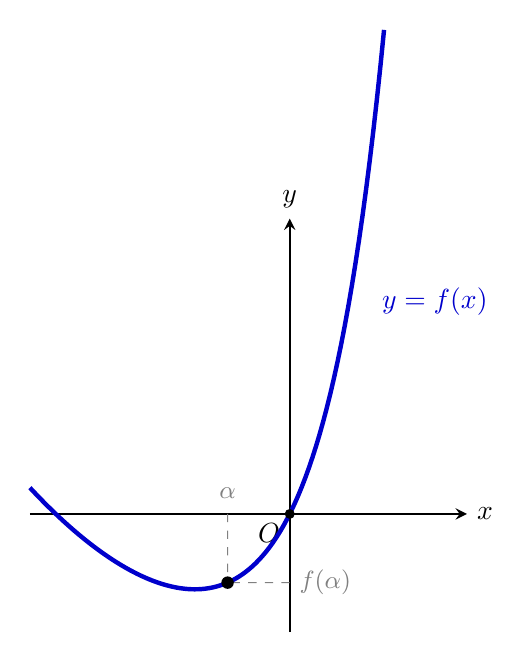
\begin{tikzpicture}[scale=1.5, >=stealth]

  % --- 1. 座標軸 ---
  \draw[->, thick] (-2.2, 0) -- (1.5, 0) node[right] {$x$};
  \draw[->, thick] (0, -1.0) -- (0, 2.5) node[above] {$y$};
  \node[below left] at (0,0) {$O$};

  % --- 2. y = f(x) の描画 (n=2 付近の定性的グラフ) ---
  % f(x) = x^2/4 + exp(2x) - 1
  % alpha ≒ -0.526
  \draw[ultra thick, blue!80!black, domain=-2.2:0.8, samples=100] 
    plot (\x, {0.25*\x*\x + exp(2*\x) - 1});
  \node[blue!80!black, right] at (0.7, 1.8) {$y = f(x)$};

  % --- 3. 極小値 alpha と解 x_n のプロット ---
  % 極小値 alpha (f'(\alpha) = 0)
  \pgfmathsetmacro{\alphaVal}{-0.526}
  \pgfmathsetmacro{\fAlpha}{0.25*\alphaVal*\alphaVal + exp(2*\alphaVal) - 1}
  \coordinate (Alpha) at (\alphaVal, \fAlpha);

  % 負の解 x_n (f(x_n) = 0, x_n != 0)
  \pgfmathsetmacro{\xn}{-1.38}
  \coordinate (Xn) at (\xn, 0);

  % --- 4. 補助線とラベル ---
  % 極小点 \alpha のガイド線
  \draw[dashed, gray] (\alphaVal, 0) node[above, font=\small, yshift=2pt] {$\alpha$} -- (Alpha);
  \draw[dashed, gray] (0, \fAlpha) node[right, font=\small] {$f(\alpha)$} -- (Alpha);
  \fill[black] (Alpha) circle (1.5pt);

  % 解 x_n のプロット
  %\fill[red!80!black] (Xn) circle (1.8pt) node[below left, font=\small] {$x_n$};

  % Y軸切片 (0, 0) - 原点を通る
  \fill[black] (0, 0) circle (1.2pt);

\end{tikzpicture}
\end{center}
\caption{$y = f(x)$ の概形}
\end{figure}

\paragraph{(2)}

$x_n$は楕円の方程式$\dfrac{x^2}{n^2}+n^2y^2=1$と$y=\dfrac{e^x}{n}$を連立した
\begin{align}
 \dfrac{1}{n^2}x_n^2+e^{2x_n}-1=0
\end{align}
の解でありかつ$x_n \neq 0$であるから，(1)より$f(x)=0$の$x\ne0$の解である．
$f(x)$の表式より
\begin{align}
 f(-n)=e^{-2n}>0 \quad\cdots\text{①} \label{eq:2}
\end{align}
である．

\begin{figure}[htb]
\begin{center}
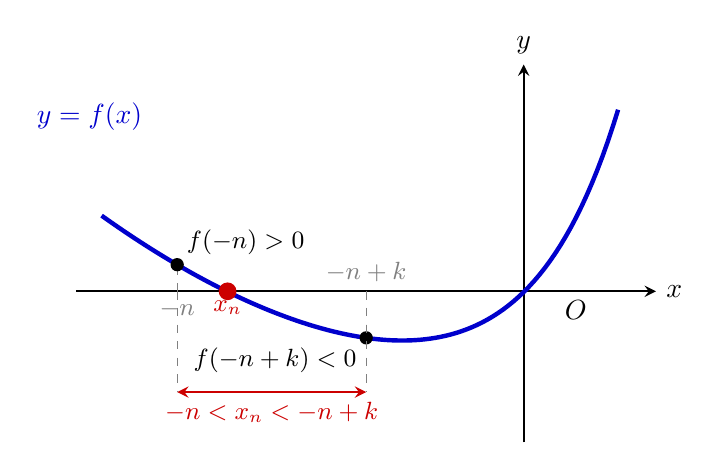
\begin{tikzpicture}[scale=1.6, >=stealth]

  % --- 1. 座標軸 ---
  \draw[->, thick] (-3.8, 0) -- (0.8, 0) node[right] {$x$};
  \draw[->, thick] (-0.25, -1.2) -- (-0.25, 1.8) node[above] {$y$};
  \node[below right] at (0,0) {$O$};

  % --- 2. y = f(x) の描画 (拡大イメージ) ---
  \draw[ultra thick, blue!80!black, domain=-3.6:0.5, samples=100] 
    plot (\x, {0.1*\x*\x + exp(1.5*\x) - 0.7});
  \node[blue!80!black, above left] at (-3.2, 1.2) {$y = f(x)$};

  % --- 3. 主要な X 座標値の設定 ---
  \def\xnVal{-2.6}    % x_n (f(x_n) = 0)
  \def\negNVal{-3.0}  % -n
  \def\negNKVal{-1.5} % -n + k

  % --- 4. 符号の正負を示す補助線 ---
  % f(-n) > 0
  \pgfmathsetmacro{\fNegN}{0.1*\negNVal*\negNVal + exp(1.5*\negNVal) - 0.7}
  \draw[dashed, gray] (\negNVal, 0) node[below, font=\small] {$-n$} -- (\negNVal, \fNegN);
  \fill[black] (\negNVal, \fNegN) circle (1.5pt) node[above right, font=\small] {$f(-n) > 0$};

  % f(-n + k) < 0
  \pgfmathsetmacro{\fNegNK}{0.1*\negNKVal*\negNKVal + exp(1.5*\negNKVal) - 0.7}
  \draw[dashed, gray] (\negNKVal, 0) node[above, font=\small] {$-n+k$} -- (\negNKVal, \fNegNK);
  \fill[black] (\negNKVal, \fNegNK) circle (1.5pt) node[below left, font=\small] {$f(-n+k) < 0$};

  % 解 x_n
  \fill[red!80!black] (\xnVal, 0) circle (2.0pt) node[below, font=\small, red!80!black] {$x_n$};

  % --- 5. 存在範囲の区間表示 ---
  \draw[<->, thick, red!80!black] (\negNVal, -0.8) -- (\negNKVal, -0.8) 
    node[midway, below, font=\small] {$-n < x_n < -n+k$};
  \draw[dashed, gray] (\negNVal, 0) -- (\negNVal, -0.8);
  \draw[dashed, gray] (\negNKVal, 0) -- (\negNKVal, -0.8);

\end{tikzpicture}
\end{center}
\caption{十分大きな $n$ における $f(-n) > 0$ および $f(-n+k) < 0$ と解 $x_n$ の位置関係}
\end{figure}



$k\, (>0)$を定数とすると
\begin{align}
\begin{split}
f(-n+k)&=\dfrac{-2kn+k^2}{n^2}+e^{2(k-n)} \\
&=-2k\cdot\dfrac{1}{n}+\dfrac{k^2}{n^2}+e^{2(k-n)}
\end{split}
\end{align}
である．
$n$が十分大きい時$\dfrac{1}{n}\gg\dfrac{1}{n^2}\gg\dfrac{1}{e^n}$だから
\begin{align}
f(-n+k)<0 \quad\cdots\text{②} \label{eq:3}
\end{align}
となる．

\cref{eq:2,eq:3}と$y=f(x)$のグラフより十分大きい$n$に対して
\begin{align}
-n<x_n<-n+k
\end{align}
である．両辺を$n\, (>0)$で割って
\begin{align}
-1<\dfrac{x_n}{n}<-1+\dfrac{k}{n}
\end{align}
となる．右辺は$n\to\infty$で$-1$に収束するからはさみうちの定理から
\begin{align}
\lim_{n\to\infty} \dfrac{x_n}{n} = -1 
\end{align}
である．



\newpage

\end{document}
